\documentclass{article}
\usepackage{subcaption}
\usepackage[labelformat=parens,labelsep=quad, skip=3pt]{caption}
\usepackage{graphicx}
\usepackage[font=small,labelfont=bf]{caption}
\usepackage{geometry}

\geometry{
 a4paper,
 left=0mm,
 top=0mm,
 }

\begin{document}



\begin{figure}[htbp]
\begin{subfigure}{.5\textwidth}
\centering
 \caption{SeaWiFS Chlorophyll}
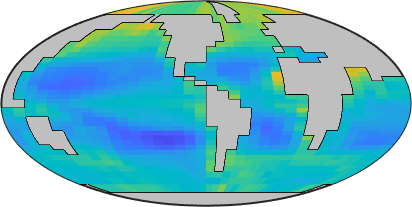
\includegraphics[width=0.95\linewidth]{Final_figures/OBSERVATIONS/SeaWiFS_on_GEnIE.png}
\end{subfigure}%
\begin{subfigure}{.5\textwidth}
\centering
 \caption{ECOGEM Chlorophyll}
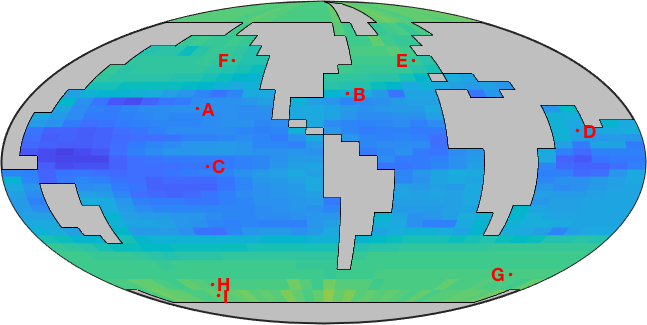
\includegraphics[width=0.95\linewidth]{Final_figures/ECOGEM/Surface_Chl_Biomass.png}
\end{subfigure}%
\\[+0.2cm]
\begin{subfigure}{.5\textwidth}
 \centering
 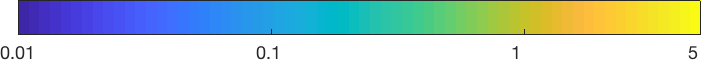
\includegraphics[width=0.95\linewidth]{Final_figures/ECOGEM/Surface_Chl_Biomass_clrbar.png}
\end{subfigure}
%%%%%
\begin{subfigure}{.5\textwidth}
\centering
 \caption{\citet{Yool:2013a} Pr. Production}
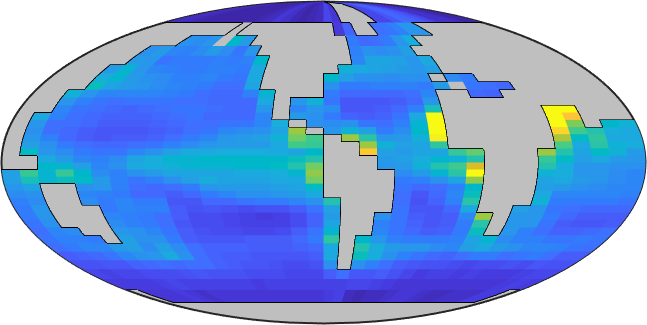
\includegraphics[width=0.95\linewidth]{Final_figures/OBSERVATIONS/Composite_PP_on_GEnIE.png}
\end{subfigure}%
\begin{subfigure}{.5\textwidth}
\centering
 \caption{ECOGEM Pr. Production}
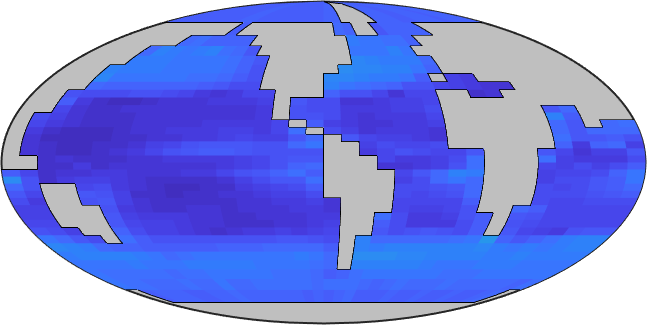
\includegraphics[width=0.95\linewidth]{Final_figures/ECOGEM/PrimaryProdn.png}
\end{subfigure}%
\\[+0.2cm]
\begin{subfigure}{.5\textwidth}
 \centering
 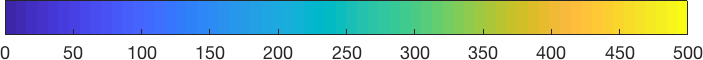
\includegraphics[width=0.95\linewidth]{Final_figures/ECOGEM/PrimaryProdn_clrbar.png}
\end{subfigure}
\caption{Satellite-derived (left) and modelled (right) surface chlorophyll~\textit{a} concentration (mg Chl m$^{-3}$) and depth-integrated primary production (mg C m$^{-2}$ d$^{-1}$). The satellite-derived estimate of primary production is a composite of three products \citep{Behrenfeld:1997,Carr:2006,Westberry:2008}, as in \citet[][their Figure~12]{Yool:2013a}.}
\label{fig:chl_prpr}
\end{figure}





\end{document}


\begin{figure}[htbp]
\begin{subfigure}{.66\textwidth}
 \centering
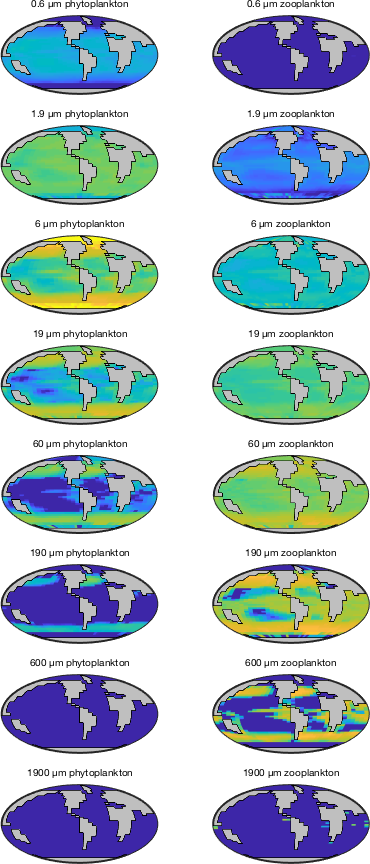
\includegraphics[width=0.8\linewidth]{Final_figures/ECOGEM/SizeClass_C_Biomass.png}
\end{subfigure} 
\\[+0.2cm]
\begin{subfigure}{.66\textwidth}
 \centering
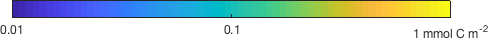
\includegraphics[width=0.8\linewidth]{Final_figures/ECOGEM/SizeClass_C_Biomass_clrbar.png}
\end{subfigure}
\caption{Surface concentrations of carbon biomass in each population (mmol C m$^{-3}$).}
\label{fig:surf_sizefrac}
\end{figure}


\begin{figure}[htbp]
\begin{subfigure}{.33\textwidth}
 \centering
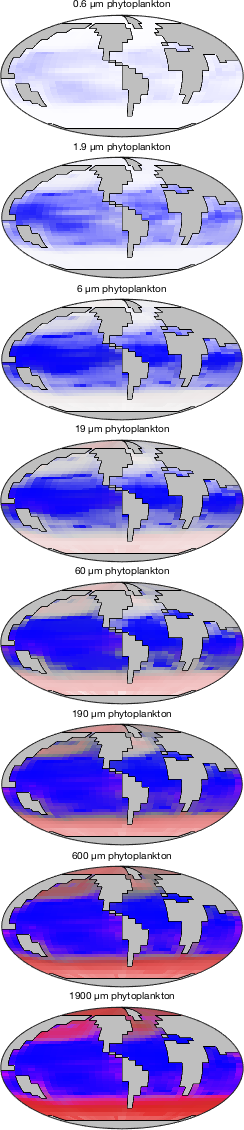
\includegraphics[width=0.95\linewidth]{Final_figures/ECOGEM/SizeClass_Limitation.png}
\end{subfigure}
\begin{subfigure}{.25\textwidth}
 \centering
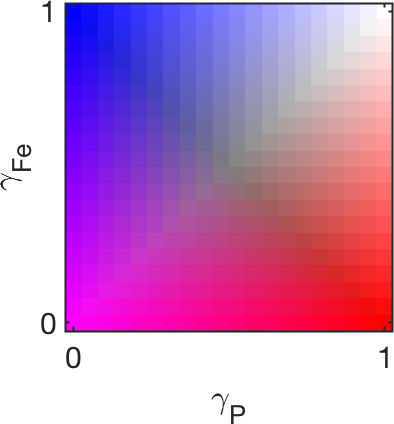
\includegraphics[width=0.95\linewidth]{Final_figures/ECOGEM/SizeClass_Limitation_clrbar.png}
\end{subfigure}
\caption{Nutrient limitation in each phytoplankton population (dimensionless). The two-dimensional colour-scale indicates decreasing phosphorus limitation from left to right, and decreasing iron limitation from bottom to top. White is therefore nutrient replete, blue is phosphorus limited, red is iron limited, and magenta is phosphorus-iron co-limited.}
\label{fig:surf_sizefrac_limitation}
\end{figure}








